\documentclass[../../main.tex]{subfiles}
\begin{document}

{\bf [解]}
接点の座標を$Q(\alpha,\alpha^2)$，$R(\beta,\beta^2)$（$\alpha<\beta$）とおく．
この時$Q,R$での接線は各々
\begin{align}
y=2\alpha x-\alpha^2, \qquad y=2\beta x-\beta^2
\end{align}
だから，この交点である$P$の座標は$\left(\dfrac{\alpha+\beta}{2},\alpha\beta\right)$である．

\begin{figure}[htb]
\begin{center}
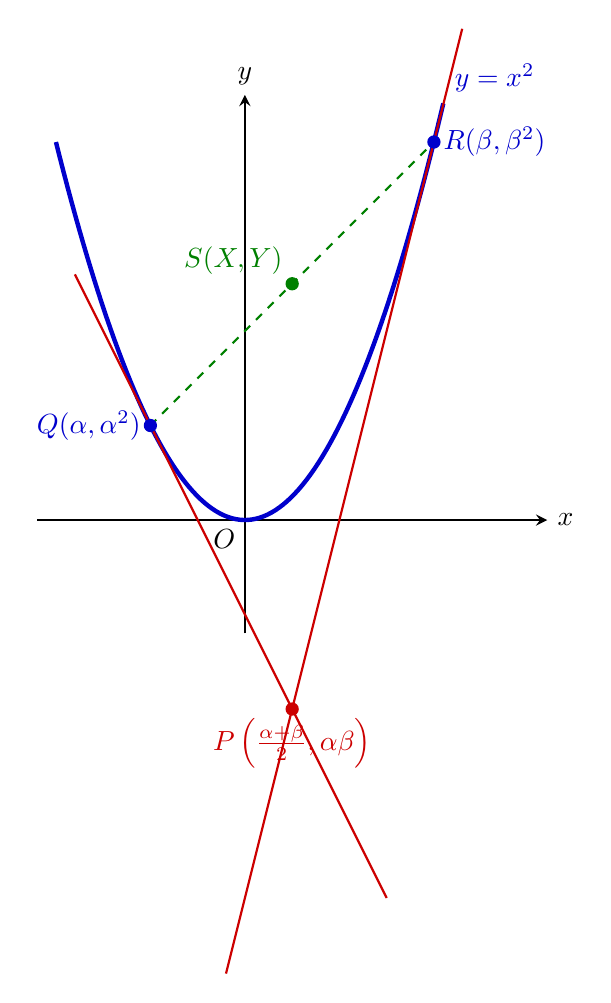
\begin{tikzpicture}[scale=1.2, >=stealth]

  % --- 1. 座標軸 ---
  \draw[->, thick] (-2.2,0) -- (3.2,0) node[right] {$x$};
  \draw[->, thick] (0,-1.2) -- (0,4.5) node[above] {$y$};
  \node[below left] at (0,0) {$O$};

  % --- 2. 放物線 y = x^2 ---
  \draw[ultra thick, blue!80!black, domain=-2.0:2.1, samples=100] 
    plot (\x, {\x*\x}) node[above right] {$y=x^2$};

  % --- 3. 点 Q, R の設定 (例: alpha = -1, beta = 2) ---
  \coordinate (Q) at (-1, 1);
  \coordinate (R) at (2, 4);

  % 交点 P ((alpha+beta)/2, alpha*beta) = (0.5, -2) の予定だが、見やすさのため yスケールに合わせて計算
  \coordinate (P) at (0.5, -2);
  
  % 中点 S ((alpha+beta)/2, (alpha^2+beta^2)/2) = (0.5, 2.5)
  \coordinate (S) at (0.5, 2.5);

  % --- 4. 2つの接線の描画 ---
  % 接線 at Q: y = 2*(-1)*x - (-1)^2 = -2x - 1
  \draw[thick, red!80!black, domain=-1.8:1.5] plot (\x, {-2*\x - 1});
  
  % 接線 at R: y = 2*(2)*x - (2)^2 = 4x - 4
  \draw[thick, red!80!black, domain=-0.2:2.3] plot (\x, {4*\x - 4});

  % --- 5. 線分 QR と中点 S ---
  \draw[thick, dashed, green!50!black] (Q) -- (R);
  \fill[green!50!black] (S) circle (2pt) node[above left] {$S(X,Y)$};

  % --- 6. 各点のプロットとラベル ---
  \fill[blue!80!black] (Q) circle (2pt) node[left] {$Q(\alpha, \alpha^2)$};
  \fill[blue!80!black] (R) circle (2pt) node[right] {$R(\beta, \beta^2)$};
  \fill[red!80!black] (P) circle (2pt) node[below] {$P\left(\frac{\alpha+\beta}{2}, \alpha\beta\right)$};

\end{tikzpicture}
\end{center}
\caption{放物線 $y=x^2$ と 2 接線・交点 $P$・中点 $S$ の位置関係}
\end{figure}


\paragraph{(1)}

題意の不等式を$\alpha,\beta$を用いて表すと
\begin{align}
\begin{cases}
 \alpha\beta \le \dfrac{\alpha+\beta}{2} - 1 \\
 \alpha\beta \le -\dfrac{\alpha+\beta}{2} + 1 \\
 -1 \le \alpha\beta  
\end{cases} \label{eq:1}
\end{align}
である．線分QRの中点$S(X,Y)$の座標は
\begin{align}
\begin{cases}
 X = \dfrac{\alpha+\beta}{2} \\
 Y = \dfrac{\alpha^2+\beta^2}{2}
\end{cases} \label{eq:2}
\end{align}
である．従って実数$\alpha,\beta\, (\alpha<\beta)$が\cref{eq:1}を満たして動く時の\cref{eq:2}の軌跡を求めれば良い．
$Y$を変形すると
\begin{align}
 2Y 
  &= \left(\alpha+\beta\right)^2 - 2\alpha\beta \\
  &= 4X^2 - 2\alpha\beta \\  
\therefore
  & \alpha\beta = 2X^2 - Y \label{eq:3}
\end{align}
だから\cref{eq:1}を$X,Y$で表すと
\begin{align}
 \begin{cases}
  2X^2 - Y \le X - 1 \\
  2X^2 - Y \le -X + 1 \\
  -1 \le 2X^2 - Y
 \end{cases} \\
\therefore
 \begin{cases}
  2X^2 - X + 1 \le Y \le 2X^2+1 \\
  2X^2 + X - 1 \le Y \le 2X^2+1 
 \end{cases} \label{eq:4}
\end{align}
である．

また$\alpha,\beta$の存在条件は二次方程式$x^2-(\alpha+\beta)x+\alpha\beta=0$の判別式$D$が正であることだから
\begin{align}
 &(\alpha+\beta)^2 - 4\alpha\beta > 0 \\
 &(2X)^2 - 4(2X^2 - Y) > 0 \\
 &Y>X^2 \label{eq:5}
\end{align}
である．

求める領域は\cref{eq:4,eq:5}である．これを図示すると下図斜線部である．

\begin{figure}[htb]
\begin{center}
\begin{tikzpicture}[scale=1.1, >=stealth]

  % --- 1. 座標軸 ---
  \draw[->, thick] (-2.7,0) -- (2.7,0) node[right] {$X$};
  \draw[->, thick] (0,-1.2) -- (0,10.2) node[above] {$Y$};
  \node[below left] at (0,0) {$O$};

  % --- 2. 領域の塗りつぶし (斜線ハッチング) ---
  % X >= 0 側: X=0 から 交点 X=2 まで (Y = 2X^2 - X - 1 から Y = 2X^2 + 1)
  \fill[pattern=north east lines, pattern color=blue!60]
    (0,1) -- plot[domain=0:2, samples=50] (\x, {2*\x*\x + 1})
    -- plot[domain=2:1, samples=50] (\x, {2*\x*\x + \x - 1}) 
    -- plot[domain=1:0, samples=50] (\x, {2*\x*\x - \x + 1}) -- cycle;


  % --- 3. 判別式条件の境界 Y = X^2 (点線・参考境界) ---
  % 領域の下側に位置し、2直線/放物線の下側境界よりもさらに下を通る
  \draw[thick, dashed, green!50!black, domain=-2.3:2.3, samples=100] 
    plot (\x, {\x*\x}) node[right] {$Y = X^2$};

  % --- 4. 境界線の描画 ---
  % (i) 上側境界 Y = 2X^2 + 1 (交点 X = ±2 まで)
  \draw[ultra thick, blue!80!black, domain=0:2.0, samples=100] 
    plot (\x, {2*\x*\x + 1}) node[above left] {$Y = 2X^2 + 1$};

  % (i) 上側境界 Y = 2X^2 + 1 (交点 X = ±2 まで)
  \draw[blue!80!black, domain=-2.1:0, samples=100] 
    plot (\x, {2*\x*\x + 1});

  % (i) 上側境界 Y = 2X^2 + 1 (交点 X = ±2 まで)
  \draw[blue!80!black, domain=2:2.1, samples=100] 
    plot (\x, {2*\x*\x + 1});


  % (ii) 下側境界 (X >= 0): Y = 2X^2 - X - 1
  \draw[ultra thick, orange!80!black, domain=0:1, samples=100] 
    plot (\x, {2*\x*\x - \x + 1}) node[right, font=\small] {$Y = 2X^2 - X + 1$};

  % (ii) 下側境界 (X >= 0): Y = 2X^2 - X - 1
  \draw[orange!80!black, domain=-1.5:0, samples=100] 
    plot (\x, {2*\x*\x - \x + 1});

  % (ii) 下側境界 (X >= 0): Y = 2X^2 - X - 1
  \draw[orange!80!black, domain=-1:2.1, samples=100] 
    plot (\x, {2*\x*\x - \x + 1});


  % (iii) 下側境界 (X < 0): Y = 2X^2 + X - 1
  \draw[ultra thick, red!80!black, domain=1:2, samples=100] 
    plot (\x, {2*\x*\x + \x - 1}) node[left, font=\small] {$Y = 2X^2 + X - 1$};

  % (iii) 下側境界 (X < 0): Y = 2X^2 + X - 1
  \draw[red!80!black, domain=-2.1:1, samples=100] 
    plot (\x, {2*\x*\x + \x - 1});

  % (iii) 下側境界 (X < 0): Y = 2X^2 + X - 1
  \draw[red!80!black, domain=2:2.1, samples=100] 
    plot (\x, {2*\x*\x + \x - 1});


  % --- 5. 交点・重要点のプロットとガイド線 ---
  % 左右の交点 (2, 9) および (-2, 9)
  \fill[black] (2, 9) circle (2pt);
  \fill[black] (-2, 9) circle (2pt);
  \fill[black] (1, 2) circle (2pt);

  
  \draw[dashed, gray] (2,0) node[below, font=\small] {$2$} -- (2,9) -- (0,9) node[left, font=\small] {$9$};
  \draw[dashed, gray] (-2,0) node[below, font=\small] {$-2$} -- (-2,9);
  \draw[dashed, gray] (1,0) node[below, font=\small] {$1$} -- (1,2) -- (0,2)  node[left, font=\small] {$2$};


  % Y 軸上の点 (0,1) および下側境界の Y 軸片 (0, -1)
  \fill[black] (0,1) circle (1.5pt) node[above left, font=\small] {$1$};
  \fill[black] (0,-1) circle (1.5pt) node[below left, font=\small] {$-1$};

  % 下側境界の頂点 (1/4, -9/8) などのガイド
  \draw[dashed, gray] (0.25,0) node[below, font=\tiny] {$\frac{1}{4}$} -- (0.25, 0.875);

\end{tikzpicture}
\caption{求める領域の図示（斜線部）}
\end{center}
\end{figure}

\paragraph{(2)}
$\overrightarrow{PQ}, \overrightarrow{PR}$は
\begin{align}
\begin{split}
 \overrightarrow{PQ}&=\left(\alpha-\dfrac{\alpha+\beta}{2},\ \alpha^2-\alpha\beta\right)=\left(\dfrac{\alpha-\beta}{2},\ \alpha(\alpha-\beta)\right) \\
 \overrightarrow{PR}&=\left(\beta-\dfrac{\alpha+\beta}{2},\ \beta^2-\alpha\beta\right)=\left(\dfrac{\beta-\alpha}{2},\ \beta(\beta-\alpha)\right)
\end{split}
\end{align}
だから，サラスの公式から三角形PQRの面積は
\begin{align}
\triangle PQR=\dfrac{1}{2}\left|\dfrac{1}{2}(\alpha-\beta)\beta(\beta-\alpha)-\dfrac{1}{2}(\beta-\alpha)\alpha(\alpha-\beta)\right|=\dfrac{1}{4}(\beta-\alpha)^3 \quad(\because\beta>\alpha) \quad\cdots\text{⑤}
\end{align}
である．題意よりこれが$2$に等しいから
\begin{align}
 2 = \dfrac{1}{4}(\beta-\alpha)^3 \quad \left(\beta-\alpha\right)^3 = 8
\end{align}
$\beta-\alpha>0$より
\begin{align}
 \beta-\alpha = 2 \label{eq:6}
\end{align}
である．これを$X,Y$で表せば良い．\cref{eq:2,eq:3}に注意すると
\begin{align}
 (\beta-\alpha)^2 
  &= (\alpha+\beta)^2 - 4\alpha\beta \\
  &= (2X)^2 - 4\left(2X^2 - Y\right) \\
  &= -4 X^2+4Y
\end{align}
だから\cref{eq:6}の二乗に代入して
\begin{align}
 &-4 X^2+4Y = 4 \\
 &Y = X^2+1
\end{align}
が求める曲線である．

\newpage

\end{document}
